\documentclass{article}

\usepackage{arxiv}
\usepackage[utf8]{inputenc} % allow utf-8 input
\usepackage[T1]{fontenc}    % use 8-bit T1 fonts
\usepackage{hyperref}       % hyperlinks
\usepackage{url}            % simple URL typesetting
\usepackage{booktabs}       % professional-quality tables
\usepackage{amsfonts}       % blackboard math symbols
\usepackage{amsmath}		% boldsymbols
\usepackage{nicefrac}       % compact symbols for 1/2, etc.
\usepackage{microtype}      % microtypography
\usepackage{lipsum}		% Can be removed after putting your text content
\usepackage{graphicx}
\usepackage[square,numbers]{natbib}
\usepackage{doi}
\usepackage{circuitikz}


\usetikzlibrary{positioning}
\usetikzlibrary{calc}

% Some useful commands
\newcommand{\ba}{\boldsymbol{a}}
\newcommand{\bb}{\boldsymbol{b}}
\newcommand{\bc}{\boldsymbol{c}}
\newcommand{\bs}{\boldsymbol{s}}
\newcommand{\0}{\boldsymbol{0}}
\newcommand{\1}{\boldsymbol{1}}
\newcommand{\cout}{c_{\mathrm{out}}}
\newcommand{\cin}{c_{\mathrm{in}}}
\newcommand{\ha}{\mathrm{ha}}
\newcommand{\fa}{\mathrm{fa}}
\newcommand{\AND}{\mathrm{and}}
\newcommand{\OR}{\mathrm{or}}
\newcommand{\NOT}{\mathrm{not}}


\title{On Noisy Additions}

\date{July 18, 2022}		% Here you can change the date presented in the paper title

\author{Ralf Herbrich \\
	Hasso-Plattner Institute\\
	Potsdam, Germany \\
	\texttt{ralf.herbrich@hpi.de} \\
}

% Uncomment to override  the `A preprint' in the header
\renewcommand{\headeright}{Technical Report}
\renewcommand{\undertitle}{Technical Report}
\renewcommand{\shorttitle}{On Noisy Additions}

%%% Add PDF metadata to help others organize their library
%%% Once the PDF is generated, you can check the metadata with
%%% $ pdfinfo template.pdf
\hypersetup{
pdftitle={On Noisy Additions},
pdfauthor={Ralf Herbrich},
pdfkeywords={electrical circuits, information theory},
}

\begin{document}
\maketitle

\begin{abstract}
	So far, most of algorithmic development has relied on the concept of {\em correct computing}, in particular at the level of the basic compute unit: the arithmetic logical unit (ALU). With the rapid rise of machine learning (ML) and artificial intelligence (AI) systems, {\em correct computing} is no longer strictly required as almost all ML and AI algorithm are based on numerical approximations of (cost) minimization problems. On the other hand, energy-efficiency is becoming increasingly important. While current research into energy-efficient ML/AI focuses on {\em approximate representations} of numbers (e.g., $k$-bit deep neural networks), we will explore the idea of {\em approximate computing} resulting out of under-powering the ALU of a processor. In this note, we will both analytically derive the distribution over integers resulting from under-powering an ALU as well as propose a number of ALU circuit designs which reduce the variation in outputs of an approximate addition. Finally, we will present real-world results of the proposed ALU concept by implementing it on a field-programmable array and comparing it to our analytical results.
\end{abstract}


% keywords can be removed
% \keywords{First keyword \and Second keyword \and More}


\section{Introduction}
Over the past 80 years, most of algorithmic development has relied on the concept of {\em correct computing}, in particular at the level of the basic compute unit: the arithmetic logical unit (ALU). This has led to incredible advancements in the field of computational architecture as well as operating systems and databases. However, with the rapid rise of machine learning (ML) and artificial intelligence (AI) algorithms, this paradigm is no longer strictly required and energy-efficiency takes a more important role. Almost all ML and AI algorithm are based on numerical approximations of (cost) minimization problems and current research into energy-efficient ML/AI focuses on {\em approximate representations} of numbers. In this note, we will explore the idea of {\em approximate computing} (see \cite{XuMytKim2022a}) starting with the simplest model of approximate additions of two integer numbers.


\section{Arithmetic Logic Units and Adders}
\label{sec:adders}
Every computer is an electric device which changes the state of its memory (i.e., randomly-accessible memory (RAM) or on-chip memory also referred to as {\em registers}) in response to the execution of instructions provided to the computer through RAM. The change of the state is performed by a unit called the {\em arithmetic logic unit} (ALU) which implements at the very least $n$-bit addition, bit-wise logic operations (i.e., AND, OR, NOT) as well as bit-wise shift operations\footnote{Computer architecture differs in the range of instructions is supports in hardware---the so-called instruction set architecture (ISA)---as well as the way that some operations are supported on RAM or only on registers.}. Note that the instructions themselves are part of the state of the computer and that the program flow through this state is handled by using the ALU on a special register called the {\em program counter} (always pointing to the location in RAM where the current instruction is contained). Thus, the ALU is the most central component that allows any computer to perform all its tasks.

\begin{figure}
    \begin{tabular}{cc}
        \begin{minipage}[c]{.45\linewidth}
            \centering
            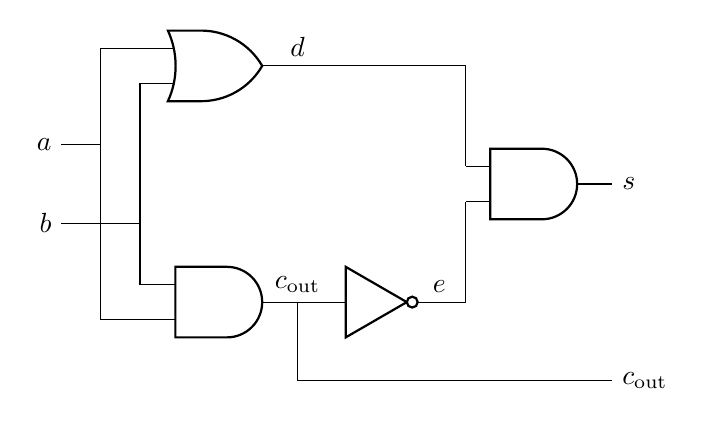
\begin{tikzpicture}
                % Circuit style
                \ctikzset{
                    logic ports=ieee,
                    logic ports/scale=0.8,
                    % logic ports/fill=lightgray
                }

                % Logic ports
                \node[or port] (OR) at (0,0){};
                \node[and port] (ANDa) at (0,-3){};
                \node[not port] (NOT) at (2,-3){};
                \node[and port] (ANDb) at (4,-1.5){};

                % Input and output ports
                \node (a) at (-2,-1) [left] {$a$};
                \node (b) at (-2,-2) [left] {$b$};
                \node (c1) at (1,-3) [above] {$\cout$};
                \node (d) at (1,0) [above] {$d$};
                \node (e) at (2.8,-3) [above] {$e$};
                \node (s) at (5,-1.5) [right] {$s$};
                \node (c2) at (5,-4) [right] {$\cout$};
                \node (af) [right = 0.5 of a, coordinate] [left] {};
                \node (bf) [right = 1 of b, coordinate] [left] {};

                % % Connection
                \draw (ANDa.out) -- (NOT.in);
                \draw (OR.out) -| (ANDb.in 1);
                \draw (NOT.out) -| (ANDb.in 2);

                \draw (ANDb.out) -* (s);
                \draw (OR.in 1) -| (af) |- (ANDa.in 2);
                \draw (OR.in 2) -| (bf) |- (ANDa.in 1);
                \draw (a) -- (af);
                \draw (b) -- (bf);
                \draw (c1) |- (c2);
            \end{tikzpicture}
        \end{minipage} &
        \begin{minipage}[c]{.5\linewidth}
            \centering
            \begin{tabular}{c|c||c|c|c|c}
                $a$ & $b$ & $d$ & $e$ & $s$ & $\cout$ \\
                \hline
                $0$ & $0$ & $0$ & $1$ & $0$ & $0$     \\
                $0$ & $1$ & $1$ & $1$ & $1$ & $0$     \\
                $1$ & $0$ & $1$ & $1$ & $1$ & $0$     \\
                $1$ & $1$ & $1$ & $0$ & $0$ & $1$     \\
            \end{tabular}
        \end{minipage}  \\
        \begin{minipage}[c]{.45\linewidth}
            \centering
            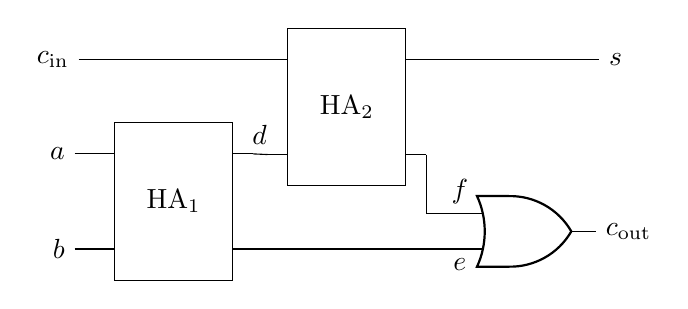
\begin{tikzpicture}
                % Circuit style
                \ctikzset{
                    logic ports=ieee,
                    logic ports/scale=0.8,
                    % logic ports/fill=lightgray
                }

                % Logic ports
                \node[draw,minimum width=1.5cm,minimum height=2cm] (HA1) at (0,-1.2){HA$_1$}
                ($(HA1.west)!0.6!(HA1.north west)$) ++(-0.25,0) coordinate (HA1in1)
                ($(HA1.west)!0.6!(HA1.south west)$) ++(-0.25,0) coordinate (HA1in2)
                ($(HA1.east)!0.6!(HA1.north east)$) ++(0.25,0) coordinate (HA1out1)
                ($(HA1.east)!0.6!(HA1.south east)$) ++(0.25,0) coordinate (HA1out2);
                \node[draw,minimum width=1.5cm,minimum height=2cm] (HA2) at (2.2,0){HA$_2$}
                ($(HA2.west)!0.6!(HA2.north west)$) ++(-0.25,0) coordinate (HA2in1)
                ($(HA2.west)!0.6!(HA2.south west)$) ++(-0.25,0) coordinate (HA2in2)
                ($(HA2.east)!0.6!(HA2.north east)$) ++(0.25,0) coordinate (HA2out1)
                ($(HA2.east)!0.6!(HA2.south east)$) ++(0.25,0) coordinate (HA2out2);
                \node[or port] (OR) at (4.5,-1.58){};

                \draw (HA1in1) -- ++(0.25,0);
                \draw (HA1in2) -- ++(0.25,0);
                \draw (HA2in1) -- ++(0.25,0);
                \draw (HA2in2) -- ++(0.25,0);
                \draw (HA1out1) -- ++(-0.25,0);
                \draw (HA1out2) -- ++(-0.25,0);
                \draw (HA2out1) -- ++(-0.25,0);
                \draw (HA2out2) -- ++(-0.25,0);

                % % Input and output ports
                \node (a)  [left = 0.25 of HA1in1] [left] {$a$};
                \node (b)  [left = 0.25 of HA1in2] [left] {$b$};
                \node (cin)[left = 2.4 of HA2in1] [left] {$\cin$};
                \node (d) [left = 0.1 of HA2in2] [above] {$d$};
                \node (e) [left = 0 of OR.in 2] [below] {$e$};
                \node (f) [left = 0 of OR.in 1] [above] {$f$};
                \node (s) [right = 2.2 of HA2out1] {$s$};
                \node (cout) [right = 0 of OR.out] [right] {$\cout$};
                \node (af) [right = 0.5 of a, coordinate] [left] {};
                \node (bf) [right = 1 of b, coordinate] [left] {};

                % % % Connection
                \draw (a) -- (HA1in1);
                \draw (b) -- (HA1in2);
                \draw (HA1out1) -- (HA2in2);
                \draw (cin) -| (HA2in1);
                \draw (HA2out2) |- (OR.in 1);
                \draw (HA1out2) |- (OR.in 2);
                \draw (HA2out1) -- (s);
            \end{tikzpicture}
        \end{minipage} &
        \begin{minipage}[c]{.5\linewidth}
            \centering
            \begin{tabular}{c|c|c||c|c|c|c|c}
                $a$ & $b$ & $\cin$ & $d$ & $e$ & $f$ & $s$ & $\cout$ \\
                \hline
                $0$ & $0$ & $0$    & $0$ & $0$ & $0$ & $0$ & $0$     \\
                $0$ & $1$ & $0$    & $1$ & $0$ & $0$ & $1$ & $0$     \\
                $1$ & $0$ & $0$    & $1$ & $0$ & $0$ & $1$ & $0$     \\
                $1$ & $1$ & $0$    & $0$ & $1$ & $0$ & $0$ & $1$     \\
                $0$ & $0$ & $1$    & $0$ & $0$ & $0$ & $1$ & $0$     \\
                $0$ & $1$ & $1$    & $1$ & $0$ & $1$ & $0$ & $1$     \\
                $1$ & $0$ & $1$    & $1$ & $0$ & $1$ & $0$ & $1$     \\
                $1$ & $1$ & $1$    & $0$ & $1$ & $0$ & $1$ & $1$     \\
            \end{tabular}
        \end{minipage}
    \end{tabular}
    \caption{{\bf Top Left:} Logic circuit design of a half-adder function that computes the sum of two binary numbers $a \in \{0,1\}$ and $b \in \{0,1\}$ where $s$ is the sum of $a$ and $b$ and $\cout$ captures the carry-bit indicating an overflow (i.e., if $a$ and $b$ are both $1$, then $s=0$ and $\cout=1$). {\bf Top Right:} The logical equivalent of the half-adder with the values for all intermediate results $d \in \{0,1\}$ and $e \in \{0,1\}$ for every possible list of (binary) input values. Note that $s = a \oplus b$ and $\cout = a \land b$. {\bf Bottom Left:} Logic circuit design of a full-adder function that computes the sum of two binary numbers $a \in \{0,1\}$ and $b \in \{0,1\}$ when a carry-in bit $\cin \in \{0,1\}$ is also passed on. {\bf Bottom Right:} The logical equivalent of the full-adder with the values for all intermediate results $d \in \{0,1\}$, $e \in \{0,1\}$ and $f \in \{0,1\}$ for every possible list of the eight (binary) input values. \label{fig:half-and-full-adder}}
\end{figure}

We will focus on one operation of the ALU that is central to all operations namely {\em addition}. Depending on the native bandwidth of the CPU, this includes the addition of two $4$-, $8$-, $16$-, $32$- or even $64$-bit numbers provided in registers. As each number is represented by bits, we will denote the two inputs to addition $A=a_0a_1a_2a_3\cdots a_n$ and $B=b_0b_1b_2b_3\cdots b_n$, respectively. The addition of $A$ and $B$ is performed in a pipeline of $n$ steps:
\begin{enumerate}
    \item {\bf Half-Adder}. First, $a_0$ and $b_0$ get added according to the rules of binary addition resulting in a sum bit $s_0$ as well as a carry-out bit $\cout^0$.
    \item {\bf Full-Adder}. Second, $a_1$, $b_1$ and $\cout^0$ get added according to the rules of binary addition with a carry-in bit $\cin^1=\cout^0$ resulting in the sum bit $s_1$ as well as the carry-out bit $\cout^1$.
    \item {\bf Ripple-Carry Adder}. This sequence is repeated until the $n$th position given the bit string $s_0s_1s_2s_3\cdots s_n\cout^n$ which is the $(n+1)$-bit answer of the addition of $A$ and $B$.
\end{enumerate}

In Figure \ref{fig:half-and-full-adder} we have shown both the circuit design as well as the logic table for a 1-bit half-adder and full-adder. In terms of logic circuits, the sum bit of the half-adder is nothing more than and XOR of both inputs $a$ and $b$ and the carry-out bit is the logical conjunction of the two inputs. For the full-adder, the sum bit is the XOR of the carry-in bit, $\cin$, and the XOR of both inputs $a$ and $b$; that is, if the carry-in bit is zero, the sum is the same as that of a half-adder but if the carry-in bit is one, the sum is the negation of the sum bit of the half-adder. Similarly, for the full-adder, the carry-out bit, $\cout$ is one if either both inputs $a$ and $b$ are one or if the carry-in bit, $\cin$ is one and at least one of $a$ and $b$ are one. More formally,
\begin{align}
    s & = a \oplus b & \cout & = a \land b \\
    s & = (a \oplus b) \oplus \cin & \cout & = (a \land b) \lor ((a \lor b) \land \cin) \label{eq:full_adder_logic} \,,
\end{align}
where the first line is for the half-adder and the second line is for the full-adder, respectively.

Looking at the rule for $\cout$ in (\ref{eq:full_adder_logic}), we can see that $(a \land b) = 1$ is {\em forcing} the carry-out bit $\cout$ to be one---irrespective of the value of $\cin$--- and that $(a \lor b) = 1$ is {\em propagating} the carry-out bit from left to right (i.e., if $\cout = \cin$). One can use these two properties when parallelizing additions over many bits because the individual conjunctions $a_i \land b_i$ do not need to wait for the carry-in bit from the prior positions (which would be required in the ripple-carry adder) and can be computed in parallel; similarly, the individual disjunctions $a_i \lor b_i$ can be computed ahead of time all that needs to happen in sequence is a correction of carry-out flags where the disjunctions were one. This circuit design is faster and is known as a {\em carry-lookahead} adder; however, we will not consider this design here.



\section{A Noise Model for Adder}
\label{sec:noisy_adders}
In this section, we are describing a noise model based on the assumption that the input voltage to the actual circuit implementing the logic NAND, NOR or NOT gates are no longer kept constant resulting in variation of the {\em actual value} of the input to the NAND, NOR or NOT unit (see \cite{LiMunPat2006l} for related work on the NOT-gate). Looking at the electrical circuit diagram of a CMOS NOT-, NAND- or NOR-gate in Figure \ref{fig:not-nand-nor-CMOS}, we see that such a variation would alter the input voltage $V_i$ thereby leading to switching behavior of the corresponding MOSFET transistors.

We assume that the random variation is fully described through two parameters $\alpha \in \left[0,\frac{1}{2}\right]$ and $\beta \in \left[0,\frac{1}{2}\right]$ which denote the probability that a low-voltage input (i.e., bit state of $0$) switches the n-type MOSFET on (i.e., bit state of $1$) and vice versa for the p-type MOSFET\footnote{Note that a flip probability of more than 50\% means that the inverted gate would make less mistakes.}. More formally, we assume that
\begin{align}
    P(a_\text{obs} = 1 | a = 0) & = \alpha\,, \label{eq:bit_flip_to_1} \\
    P(a_\text{obs} = 0 | a = 1) & = \beta\,. \label{eq:bit_flip_to_0}
\end{align}
With this noise model, it is possible that an NAND, NOR or NOT gate make mistakes in their computation. In the following table, we have listed the respective probability of each outcome $0$ and $1$ for the full list of bit-wise inputs $a$ and $b$.

\begin{center}
    \begin{tabular}{c|c||c|c||c|c||c|c}
        \multicolumn{2}{c||}{}         &
        $P\left(a \land b = 1\right)$  & $P\left(a \land b = 0\right)$  &
        $P\left(a \lor b = 1\right)$   & $P\left(a \lor b = 0\right)$   &
        $P\left(\neg a = 0\right)$     & $P\left(\neg a = 1\right)$       \\
        \hline
        $a$                            & $b$                            &
        $q_\NAND(a,b,0)$               & $q_\NAND(a,b,1)$               &
        $q_\NOR(a,b,0) $               & $q_\NOR(a,b,1)$                &
        $q_\NOT(a,0)$                  & $q_\NOT(a,1)$                    \\
        \hline
        $0$                            & $0$                            &
        $\alpha^2$                     & $1-\alpha^2$                   &
        $1-\left(1-\alpha\right)^2$    & $\left(1-\alpha\right)^2$      &
        $\alpha$                       & $1-\alpha$                       \\
        $0$                            & $1$                            &
        $\alpha\left(1-\beta\right)$   & $1-\alpha\left(1-\beta\right)$ &
        $1-\left(1-\alpha\right)\beta$ & $\left(1-\alpha\right)\beta$   &
        $\alpha$                       & $1-\alpha$                       \\
        $1$                            & $0$                            &
        $\alpha\left(1-\beta\right)$   & $1-\alpha\left(1-\beta\right)$ &
        $1-\left(1-\alpha\right)\beta$ & $\left(1-\alpha\right)\beta$   &
        $1-\beta$                      & $\beta$                          \\
        $1$                            & $1$                            &
        $\left(1-\beta\right)^2$       & $1-\left(1-\beta\right)^2$     &
        $1-\beta^2$                    & $\beta^2$                      &
        $1-\beta$                      & $\beta$                          \\
    \end{tabular}
\end{center}
% \vspace{1em}

Note that this probability distribution reduces to point functions for $\alpha = \beta = 0$. Also, for $\alpha = \beta = \frac{1}{2}$, there is {\em still} information in the computation as the resulting probability distributions for NAND and NOR are {\em not} uniform: for NAND there are three bit patterns where $\neg(a \land b)$ equals one and only one bit pattern where $\neg(a \land b)$ equals zero and thus, for truly random bit flips there is a three times larger probability that the value of the NAND computation is one than zero; $P(\neg(a \land b) = 1)=\frac{3}{4}=3\cdot P(\neg(a \land b) = 0)=\frac{1}{4}$. A similar argument applies to NOR but with the event probabilities reversed. Only the NOT function is truly uniform if $\alpha = \beta = \frac{1}{2}$.

\paragraph{Noise Half Adders} Given the logic circuit design in the top row of Figure \ref{fig:half-adder}, we can now compute the marginal distribution over the sum bit $s$ and the carry-out bit $\cout$ of a half-adder by summing over all possible values of $d \in \Bin$, $e \in \Bin$, $f \in \Bin$ and $g \in \Bin$ using the probability distributions given above. More formally, we have
\begin{align}
    P(s,\cout|a,b) & = \sum_{d\in\mathbb{B}} \sum_{e\in\mathbb{B}} \sum_{f\in\mathbb{B}} \sum_{g\in\mathbb{B}} P(s,\cout,d,e,f,g|a,b) \nonumber                                                                                              \\
                   & = \sum_{d\in\mathbb{B}} \sum_{e\in\mathbb{B}} \sum_{f\in\mathbb{B}} \sum_{g\in\mathbb{B}} P(d|a,b)\cdot P(e|a,b) \cdot P(f|d) \cdot (g|e,f) \cdot P(s|g) \cdot P(\cout|e) \nonumber                                     \\
                   & = \sum_{d\in\mathbb{B}} P(d|a,b) \cdot \sum_{e\in\mathbb{B}} P(e|a,b) \cdot P(\cout|e) \cdot  \sum_{f\in\mathbb{B}} P(f|d) \cdot \sum_{g\in\mathbb{B}}  (g|e,f) \cdot P(s|g)  \nonumber                                 \\
                   & = \sum_{d\in\mathbb{B}} q_\NOR(a,b,d) \cdot \sum_{e\in\mathbb{B}} q_\NAND(a,b,e) \cdot q_\NOT(e,\cout) \cdot \sum_{f\in\mathbb{B}} q_\NOT(d,f) \cdot \sum_{g\in\mathbb{B}}  q_\NAND(e,f,g) \cdot q_\NOT(g,s)  \nonumber \\
                   & =: q_\ha(a,b,s,\cout) \label{eq:noisy_half_adder} \,,
\end{align}
where the first line follows from the law of total probability, the second line follows from the directed graphical network structure of the half-adder, the third line follows from pulling out each of the terms as far as possible from the inner sums, and the last line follows from the definition of the probabilistic logic gates. Note that in an efficient implementation, the partial sums after summing out $g \in \mathbb{B}$, $f \in \mathbb{B}$, and $e \in \mathbb{B}$ are the so-called {\em messages} in the factor graph of logic circuit functions (see \cite{KscFreLoe2001y} for a full overview of message passing).

\paragraph{Noisy Full Adders} Using (\ref{eq:noisy_half_adder}) and the logic circuit design of the full-adder in Figure \ref{fig:full-adder}, we can now compute the marginal distribution over the sum bit $s$ and the carry-out bit $\cout$ of a full-adder by summing over all possible values of $d \in \Bin$, $e \in \Bin$, $f \in \Bin$ and $g \in \Bin$. We have
\begin{align}
    P_\fa(s,\cout|a,b,\cin) & = \sum_{d\in\mathbb{B}} \sum_{e\in\mathbb{B}} \sum_{f\in\mathbb{B}} \sum_{g\in\mathbb{B}} P(s,\cout,d,e,f,g|a,b,\cin) \nonumber                                                      \\
                            & = \sum_{d\in\mathbb{B}} \sum_{e\in\mathbb{B}} \sum_{f\in\mathbb{B}} \sum_{g\in\mathbb{B}}
    P(d,e|a,b) \cdot P(s,f|\cin,d) \cdot P(g|e,f) \cdot P(\cout|g) \nonumber                                                                                                                                       \\
                            & = \sum_{d\in\mathbb{B}} \sum_{e\in\mathbb{B}} P(d,e|a,b) \cdot \sum_{f\in\mathbb{B}} P(s,f|\cin,d) \cdot \sum_{g\in\mathbb{B}} P(g|e,f) \cdot P(\cout|g) \nonumber                   \\
                            & = \sum_{d\in\mathbb{B}} \sum_{e\in\mathbb{B}} q_\ha(a,b,d,e) \cdot \sum_{f\in\mathbb{B}} q_\ha(\cin,d,s,f) \cdot \sum_{g\in\mathbb{B}} q_\NOR(e,f,g) \cdot q_\NOT(g,\cout) \nonumber \\
                            & =: q_\fa(a,b,\cin,s,\cout) \label{eq:noisy_full_adder} \,,
\end{align}
where the first line follows from the law of total probability, the second line follows from the directed graphical network structure of the full-adder, the third line follows again from pulling out each of the terms as far as possible from the inner sums, and the last line follows from the definition of the probabilistic logic gates. Again, in an efficient implementation the probability distribution table $q_\ha \in \mathbb{R}^{\Bin\times\Bin\times\Bin\times\Bin}$ of the half-adder is computed once and re-used in all the inner sums.

\paragraph{Noisy $4$-bit Adders} Finally, using (\ref{eq:noisy_half_adder}) and (\ref{eq:noisy_full_adder}), we can compute the marginal distribution over the output $S:=s_0s_1s_2s_3\cout^3$ of a $4$-bit adder of $A$ and $B$ by summing over all possible values of $\cout^0$, $\cout^1$ and $\cout^2$. We have
\begin{align}
    P(S|A,B) & = \sum_{\cout^0 \in \Bin} \sum_{\cout^1\in\Bin} \sum_{\cout^2\in\Bin} P(s_0,s_1,s_2,s_3,\cout^0,\cout^1,\cout^2,\cout^3|A,B) \nonumber                                                          \\
             & = \sum_{\cout^0 \in \Bin} \sum_{\cout^1\in\Bin} \sum_{\cout^2\in\Bin} P(s_0,\cout^0|a_0,b_0)P(s_1,\cout^1|a_1,b_1,\cout^0)\cdots P(s_3,\cout^3|a_1,b_1,\cout^2) \nonumber                       \\
             & = \sum_{\cout^0 \in \Bin} \sum_{\cout^1\in\Bin} \sum_{\cout^2\in\Bin} q_\ha(a_0,b_0,s_0,\cout^0)\cdot q_\fa(a_1,b_1,\cout^0,s_1,\cout^1)\cdots q_\fa(a_1,b_1,\cout^2,s_3,\cout^3) \nonumber \,,
\end{align}
where the second line follows from the (chain) directed graphical network structure of the 4-bit adder. Again, we use the  pre-computed functions $q_\ha$ and $q_\fa$ for a fast computation of the output distribution of the 4-bit adder.

\begin{figure}
    \begin{tabular}{ccc}
        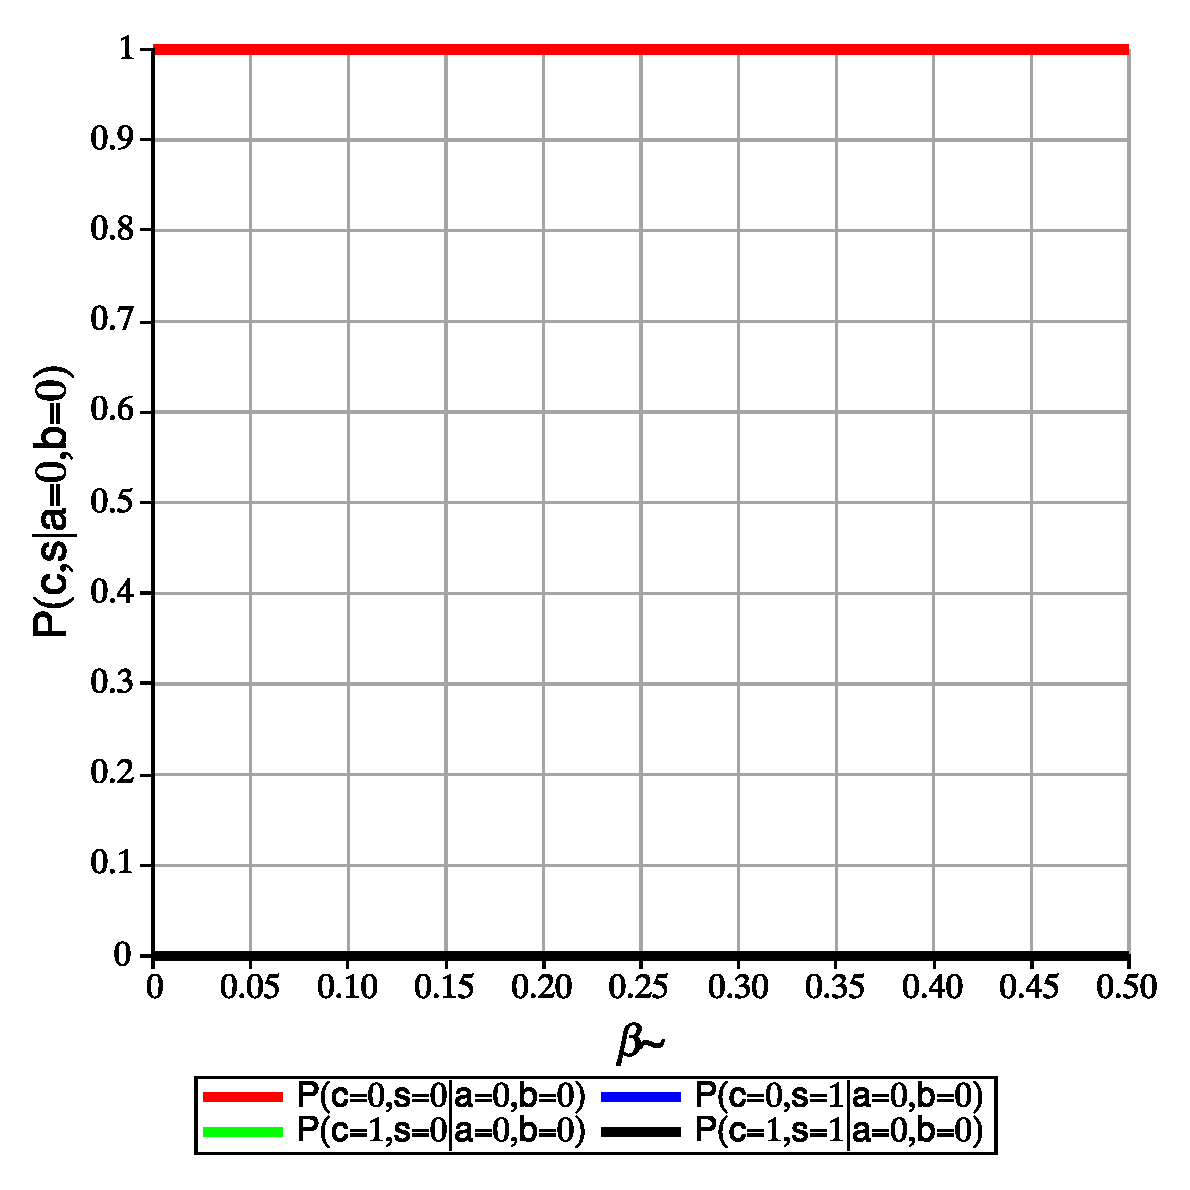
\includegraphics[width=.3\textwidth]{media/noisy_half_adder_value_dist_00.eps}  &
        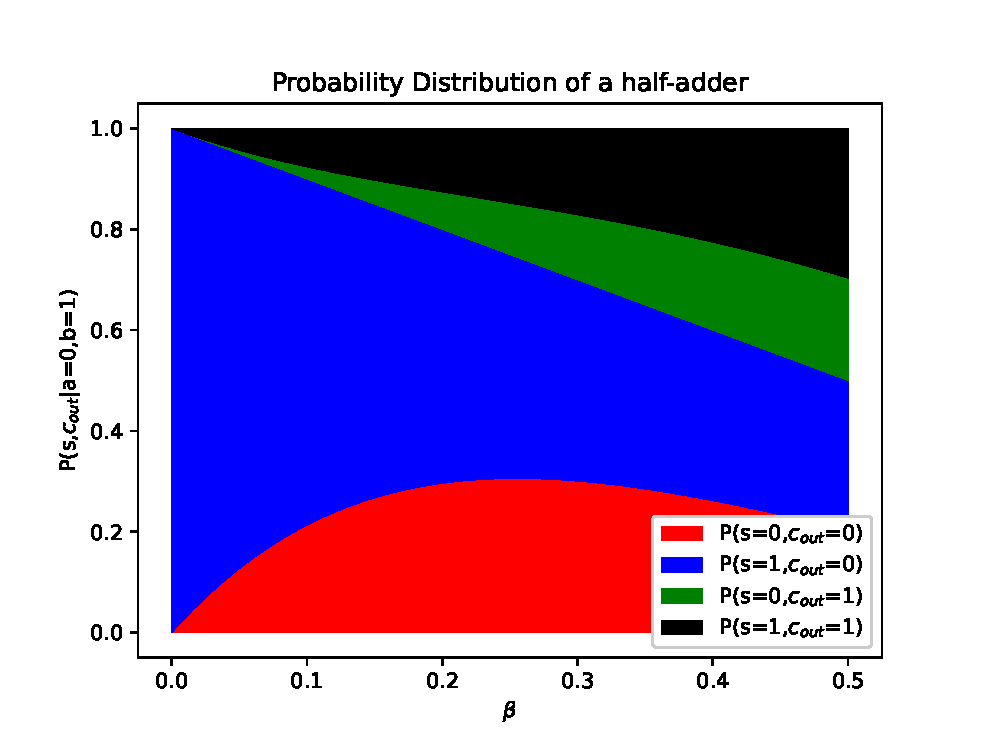
\includegraphics[width=.3\textwidth]{media/noisy_half_adder_value_dist_01.eps}  &
        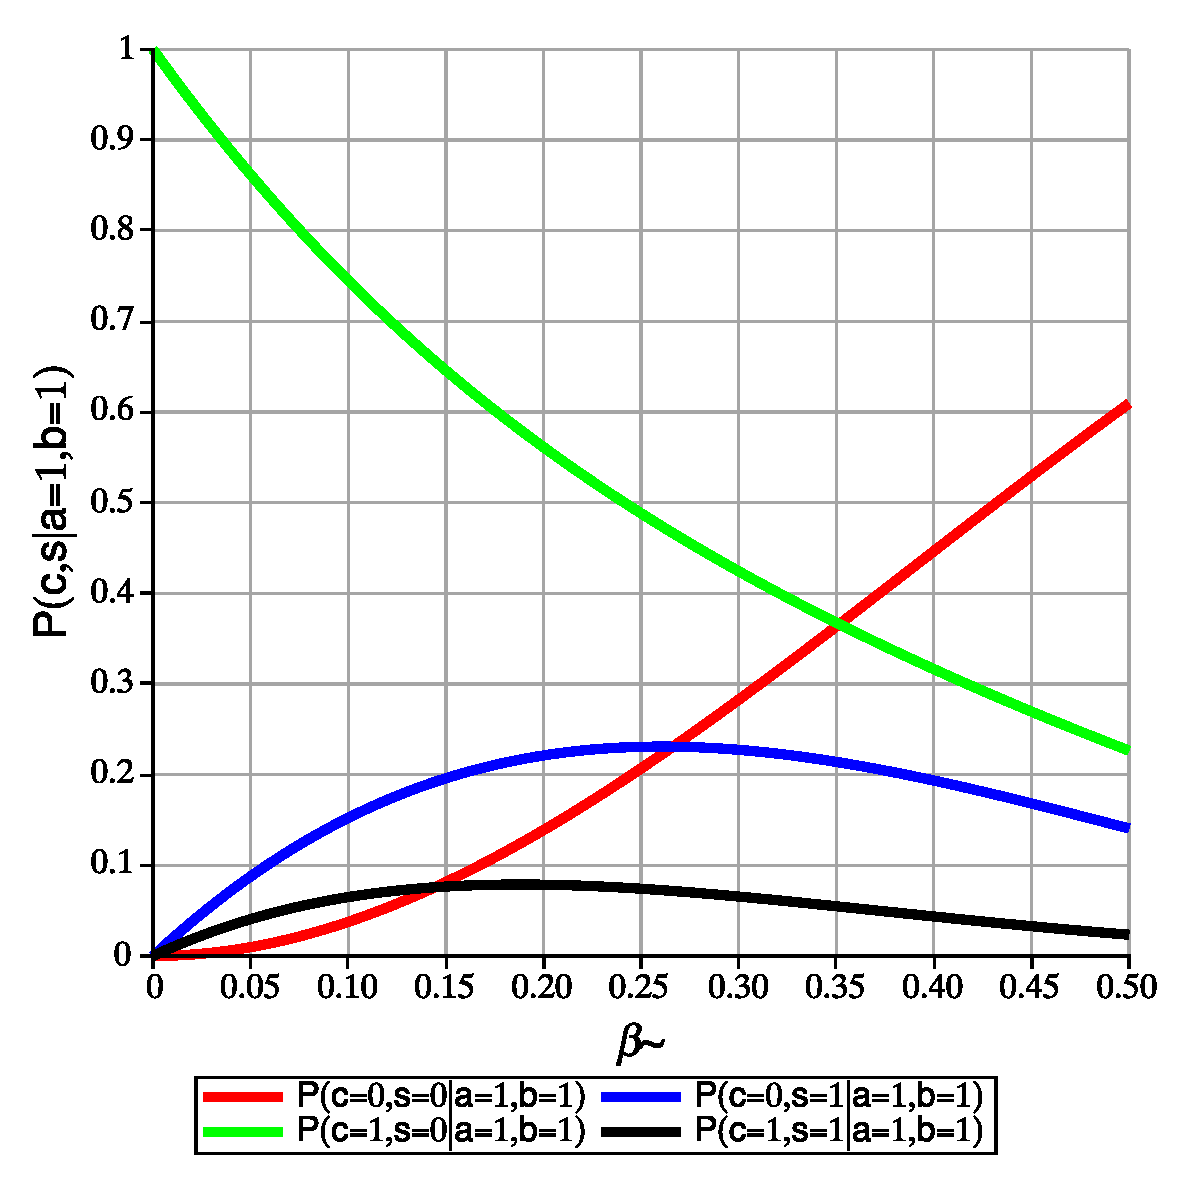
\includegraphics[width=.3\textwidth]{media/noisy_half_adder_value_dist_11.eps}    \\
        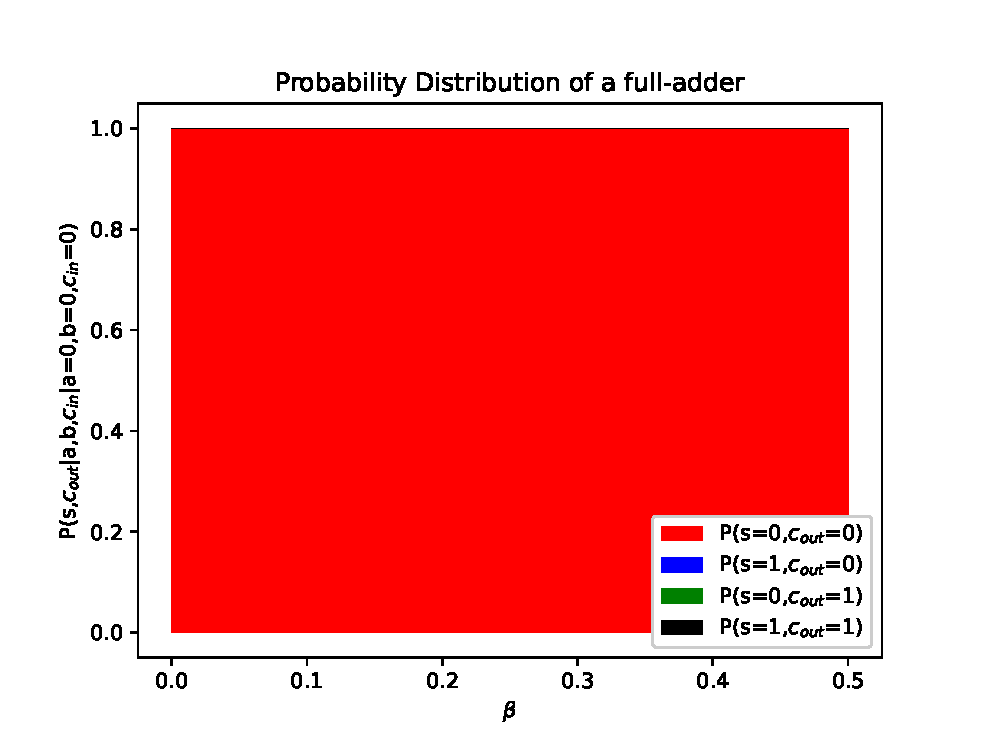
\includegraphics[width=.3\textwidth]{media/noisy_full_adder_value_dist_000.eps} &
        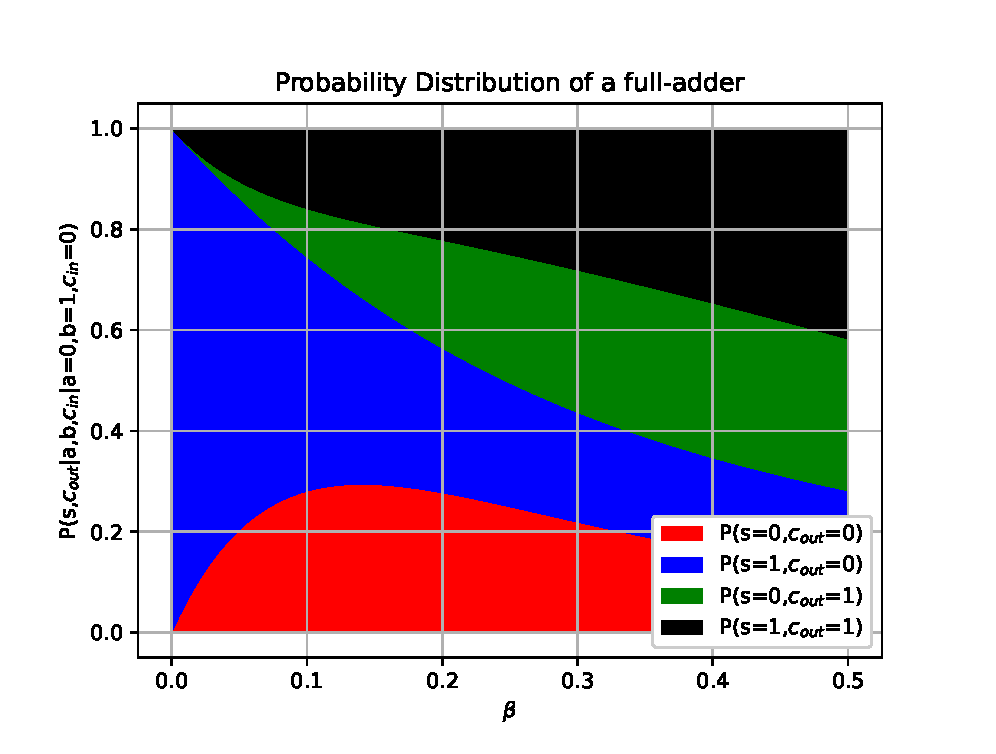
\includegraphics[width=.3\textwidth]{media/noisy_full_adder_value_dist_010.eps} &
        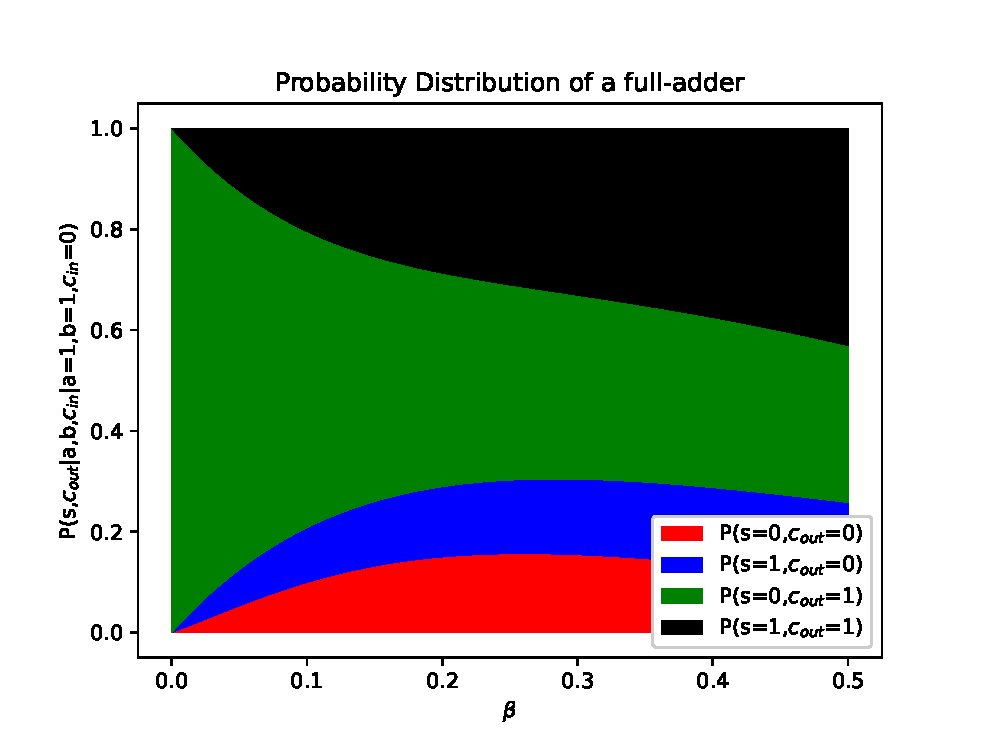
\includegraphics[width=.3\textwidth]{media/noisy_full_adder_value_dist_110.eps}   \\
        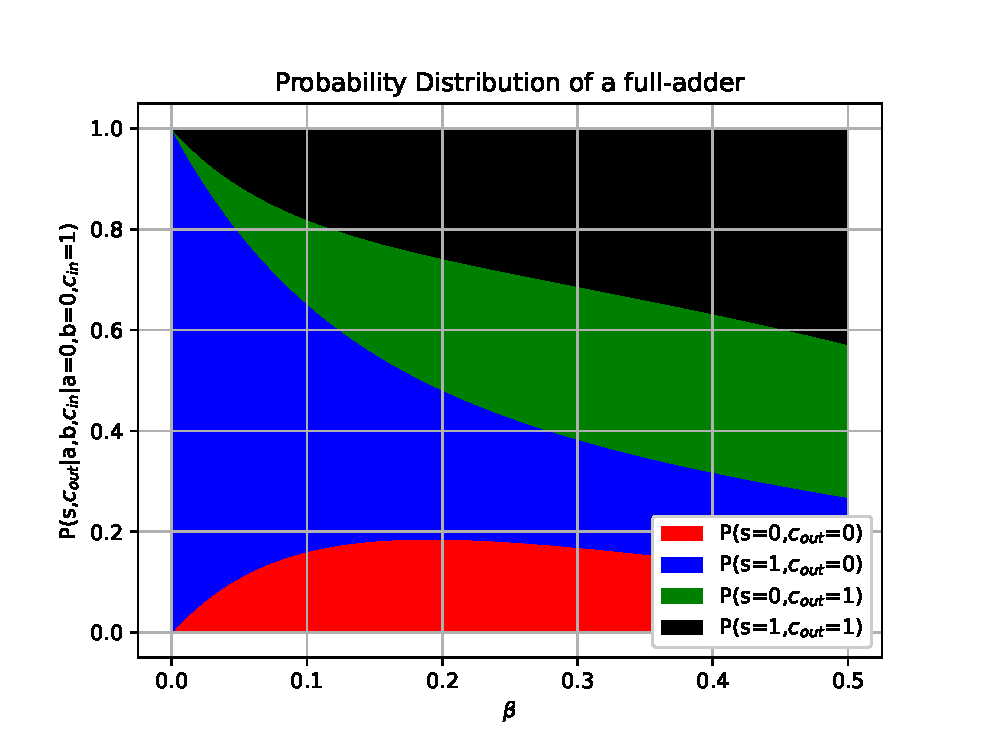
\includegraphics[width=.3\textwidth]{media/noisy_full_adder_value_dist_001.eps} &
        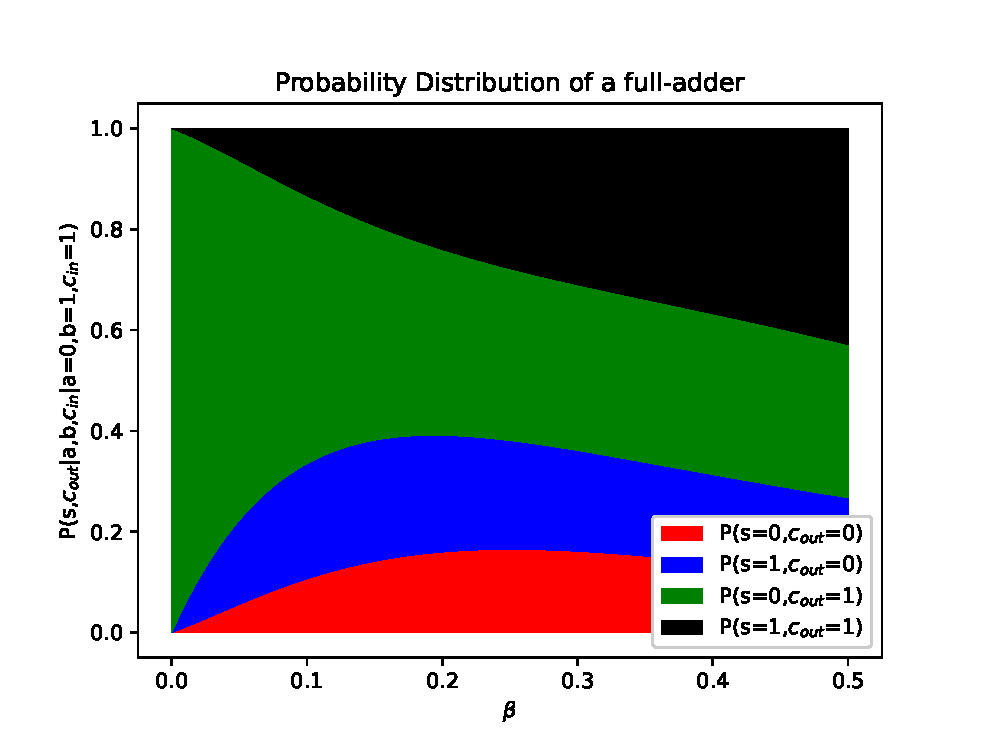
\includegraphics[width=.3\textwidth]{media/noisy_full_adder_value_dist_011.eps} &
        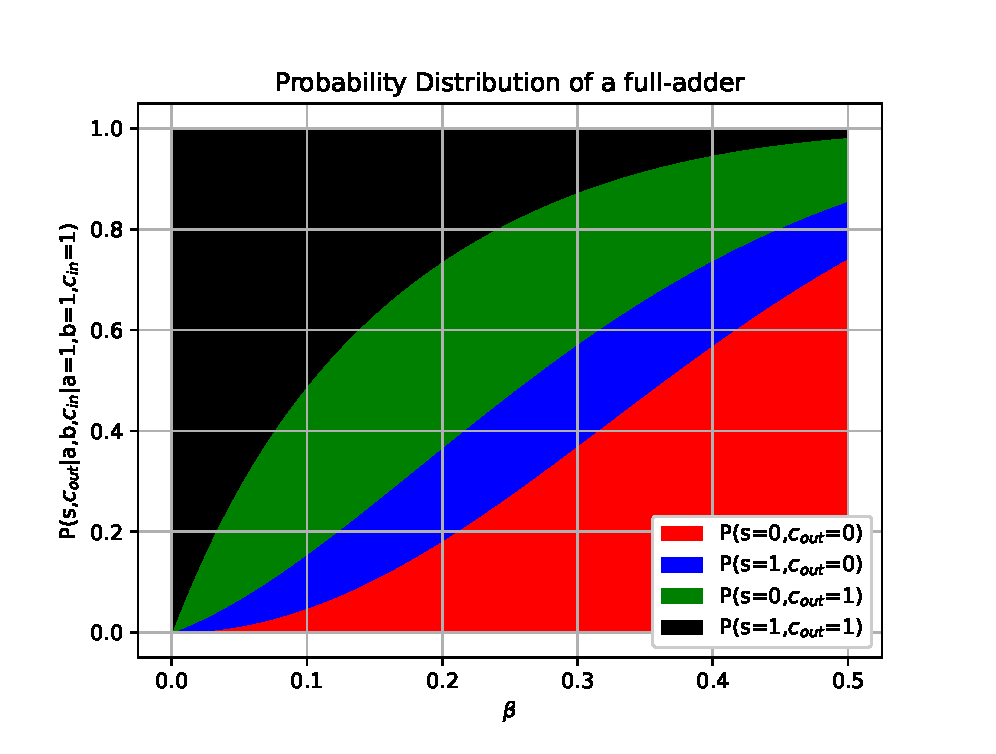
\includegraphics[width=.3\textwidth]{media/noisy_full_adder_value_dist_111.eps}   \\
    \end{tabular}
    \caption{Probability distribution for $P(s,\cout)$ for all distinct inputs for the noisy half-adder (top row) and the full-adder (middle \& bottom row). The graphs show the change of the probability distributions over the four possible outcomes as stack-plots as $\beta$ in (\ref{eq:bit_flip_to_0}) varies from $0$ to $\frac{1}{2}$ and $\alpha = 0$; this case is equivalent to assuming there is only leakage of information due to low-voltage. In all graphs, red denotes $P(s=0,\cout=0)$, blue denotes $P(s=1,\cout=1)$, green denote $P(s=0,\cout=1)$ and black denotes $P(s=1,\cout=1)$. Note that longer computation paths bias towards more errors, for example the plots in the top and middle row should be identical because they have the same truth table. \label{fig:noise_prob_dist}}
\end{figure}

In Figure \ref{fig:noise_prob_dist} we have shown how the distributions of the half-adder and full-adder vary as functions of $\beta$ when $\alpha=0$ (i.e., it is not possible that any of the input bits ever flip erroneously from $0$ to $1$). Similarly, in Figure \ref{fig:noise_prob_dist_4bit_adder} we have shown the distribution of the sum for the 4-bit adder for different values of $\beta$. One thing to note about this induced probability distribution is that, the longer the computation path, the more errors get introduced: for example, the top and middle row of Figure \ref{fig:noise_prob_dist} should have identical distributions as their truth tables are identical but the middle row uses more logic gates as an additional half-adder is used. Also, while the variance of the noisy 4-bit adder is somewhat symmetric, but for more than 10\% of bit-flip noise the right output is not always the most likely anymore.

\begin{figure}
    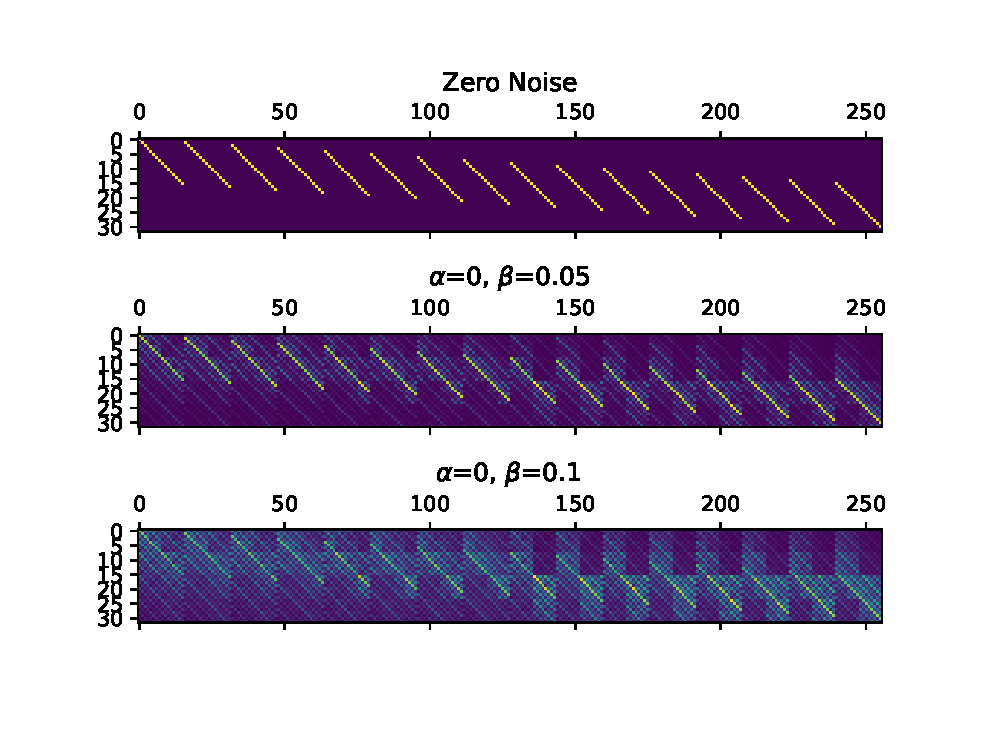
\includegraphics[width=.95\textwidth]{media/noisy_4bit_adder_value_dist_full.eps}
    \caption{Probability distribution for $P(S|A,B)$ for all distinct 256 inputs for the noisy 4-bit adder for increasing values of the noise $\beta$ in (\ref{eq:bit_flip_to_0}). In each of the 3 plots, $S$ takes up to 31 values indexing the $y$-axis and $(A,B)$ take up to 256 values (i.e., the bit-string $a_0a_1a_2a_3b_0b_1b_2b_3$ interpreted as an 8-byte number). \label{fig:noise_prob_dist_4bit_adder}}
\end{figure}



\section{k--Redundant Approximate Adders}
\label{sec:redundant_adders}
The source of the errors of the noisy addition is the error rate of the AND, OR and NOT gates; for example, with probability $1-(1-\beta)^2$ the carry bit $c=0$ even when $a=1$ and $b=1$. In order to reduce this error probability of the AND and OR gates, we propose to introduce scalable {\em redundant computation} (similar to the idea of redundancy in messages in order to compensate for channel noise in communication, see, e.g.\ \cite{Sha1948k}). One such idea is to {\em duplicate} the original function and combine the two parallel computations with an OR such that a value of $1$ is computed if at least one of the original units computes a $1$. More formally, we define
\begin{align}
    a \land_2 b & = (a \land b) \lor (a \land b) \\
    a \lor_2 b & = (a \lor b) \lor (a \lor b) \,.
\end{align}
This type of redundancy will achieve the desired effect of minimizing the error of not computing $1$. Similarly, we can combine the original units with and AND gate which minimized the error of not computing $0$. 

Using this design pattern, we can now increase the redundancy in an exponential fashion by virtue of 
\begin{align}
    a \land_{2k} b & = (a \land_k b) \lor (a \land_k b) \\
    a \lor_{2k} b & = (a \lor_k b) \lor (a \lor_k b) \,.
\end{align}
Note that this design still uses the original noise OR gate to compute the combination of all outputs. In Figure \ref{fig:noise_prob_dist_redudancy} we have shown the new probability distribution over the four possible values of $(s,c)$ when replacing all the AND and OR gates in Figure \ref{fig:half-and-full-adder} with $16$--redundant AND and OR gates. All the way to $\beta \approx 10\%$, the error remains relatively small compared to the noise-free half-adder!

\begin{figure}
    \begin{minipage}[c]{.45\linewidth}
        \centering
        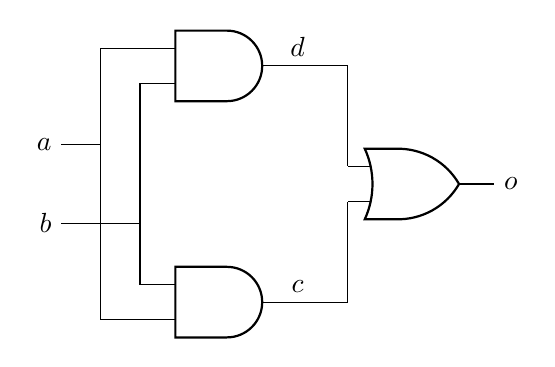
\begin{tikzpicture}
            % Circuit style
            \ctikzset{
                logic ports=ieee,
                logic ports/scale=0.8,
                % logic ports/fill=lightgray
            }

            % Logic ports
            \node[and port] (ANDa) at (0,0){};
            \node[and port] (ANDb) at (0,-3){};
            \node[or port] (OR) at (2.5,-1.5){};

            % Input and output ports
            \node (a) at (-2,-1) [left] {$a$};
            \node (b) at (-2,-2) [left] {$b$};
            \node (c) at (1,-3) [above] {$c$};
            \node (d) at (1,0) [above] {$d$};
            \node (s) at (3.5,-1.5) [right] {$o$};
            \node (af) [right = 0.5 of a, coordinate] [left] {};
            \node (bf) [right = 1 of b, coordinate] [left] {};

            % % Connection
            \draw (ANDa.out) -| (OR.in 1);
            \draw (ANDb.out) -| (OR.in 2);

            \draw (OR.out) -* (s);
            \draw (ANDa.in 1) -| (af) |- (ANDb.in 2);
            \draw (ANDa.in 2) -| (bf) |- (ANDb.in 1);
            \draw (a) -- (af);
            \draw (b) -- (bf);
        \end{tikzpicture}
    \end{minipage} \hfill
    \begin{minipage}[c]{.45\linewidth}
        \centering
        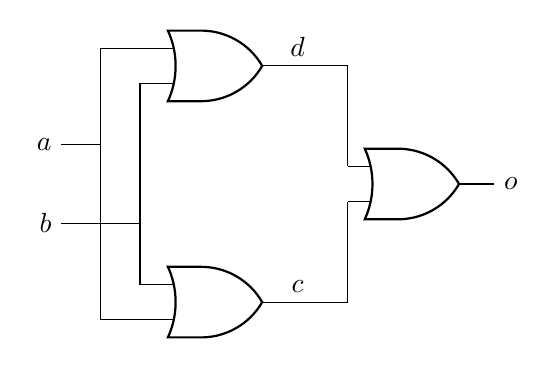
\begin{tikzpicture}
            % Circuit style
            \ctikzset{
                logic ports=ieee,
                logic ports/scale=0.8,
                % logic ports/fill=lightgray
            }

            % Logic ports
            \node[or port] (ORa) at (0,0){};
            \node[or port] (ORb) at (0,-3){};
            \node[or port] (OR) at (2.5,-1.5){};

            % Input and output ports
            \node (a) at (-2,-1) [left] {$a$};
            \node (b) at (-2,-2) [left] {$b$};
            \node (c) at (1,-3) [above] {$c$};
            \node (d) at (1,0) [above] {$d$};
            \node (s) at (3.5,-1.5) [right] {$o$};
            \node (af) [right = 0.5 of a, coordinate] [left] {};
            \node (bf) [right = 1 of b, coordinate] [left] {};

            % % Connection
            \draw (ORa.out) -| (OR.in 1);
            \draw (ORb.out) -| (OR.in 2);

            \draw (OR.out) -* (s);
            \draw (ORa.in 1) -| (af) |- (ORb.in 2);
            \draw (ORa.in 2) -| (bf) |- (ORb.in 1);
            \draw (a) -- (af);
            \draw (b) -- (bf);
        \end{tikzpicture}
    \end{minipage}
    \caption{{\bf Left:} Logic circuit design of a $2$--redundant AND gate that computes the function $a \land_2 b := (a \land b) \lor (a \land b)$ which has the exact same truth table than $a \land b$. However, this design has the property that for noisy computations, the probability of erroneously computing $1 \land 1$ as $0$ is reduced when summing out all the four values of $(c,d)$. {\bf Right:} Logic circuit design of a $2$--redundant OR gate that computes the function $a \lor_2 b := (a \lor b) \lor (a \lor b)$ which has the exact same truth table than $a \lor b$.}
\end{figure}

\begin{figure}
    \begin{center}
        \begin{tabular}{cc}
            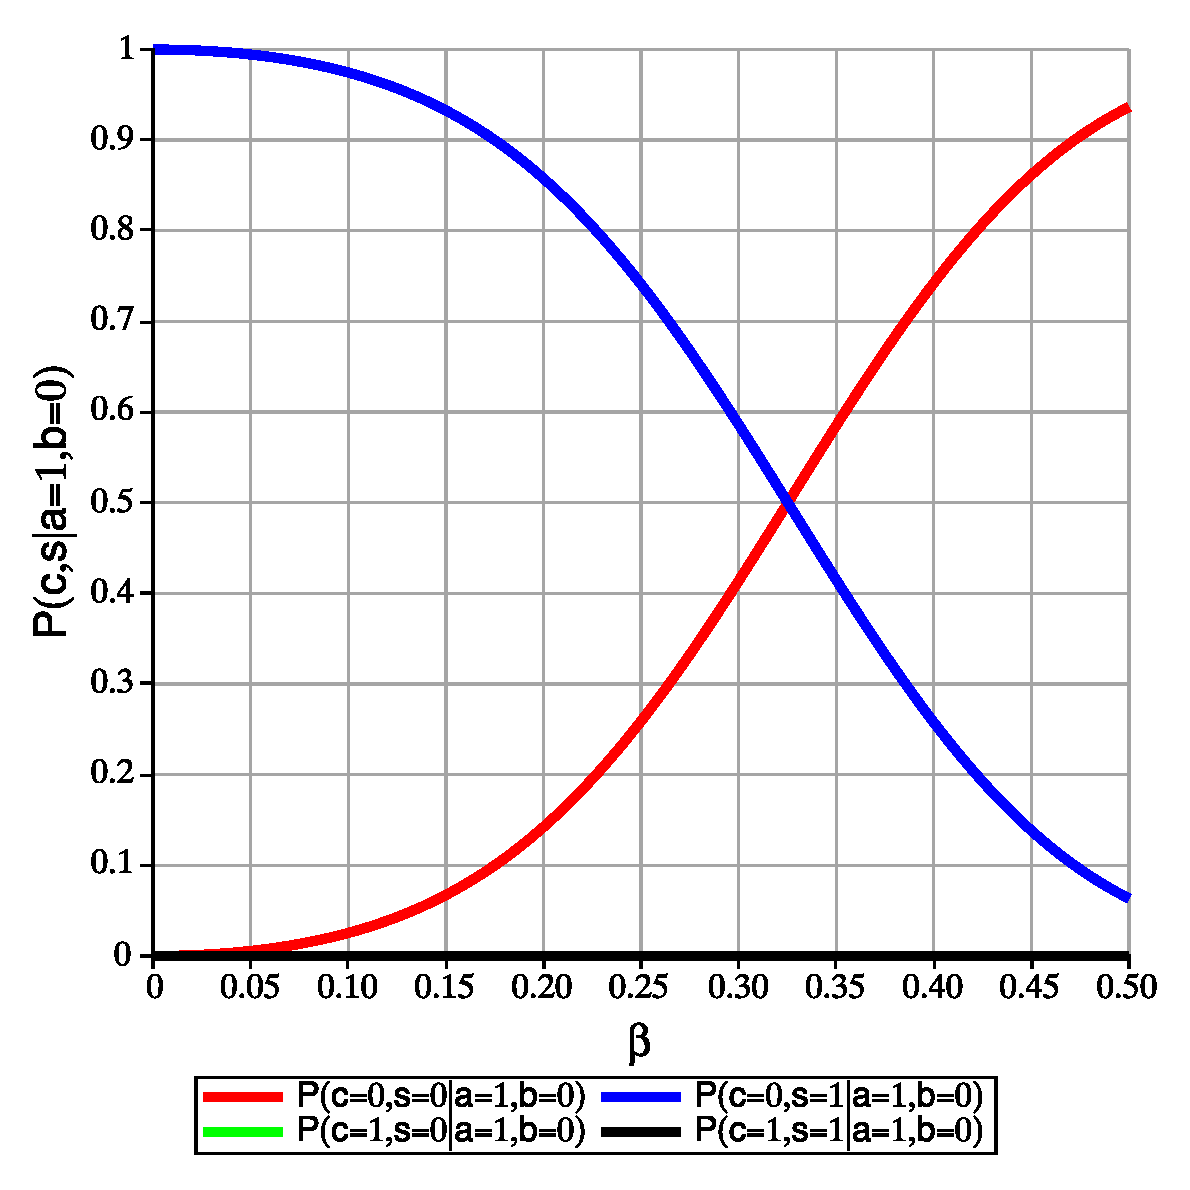
\includegraphics[width=.4\textwidth]{media/noisy_half_adder_16_redundancy_value_dist_10.eps} &
            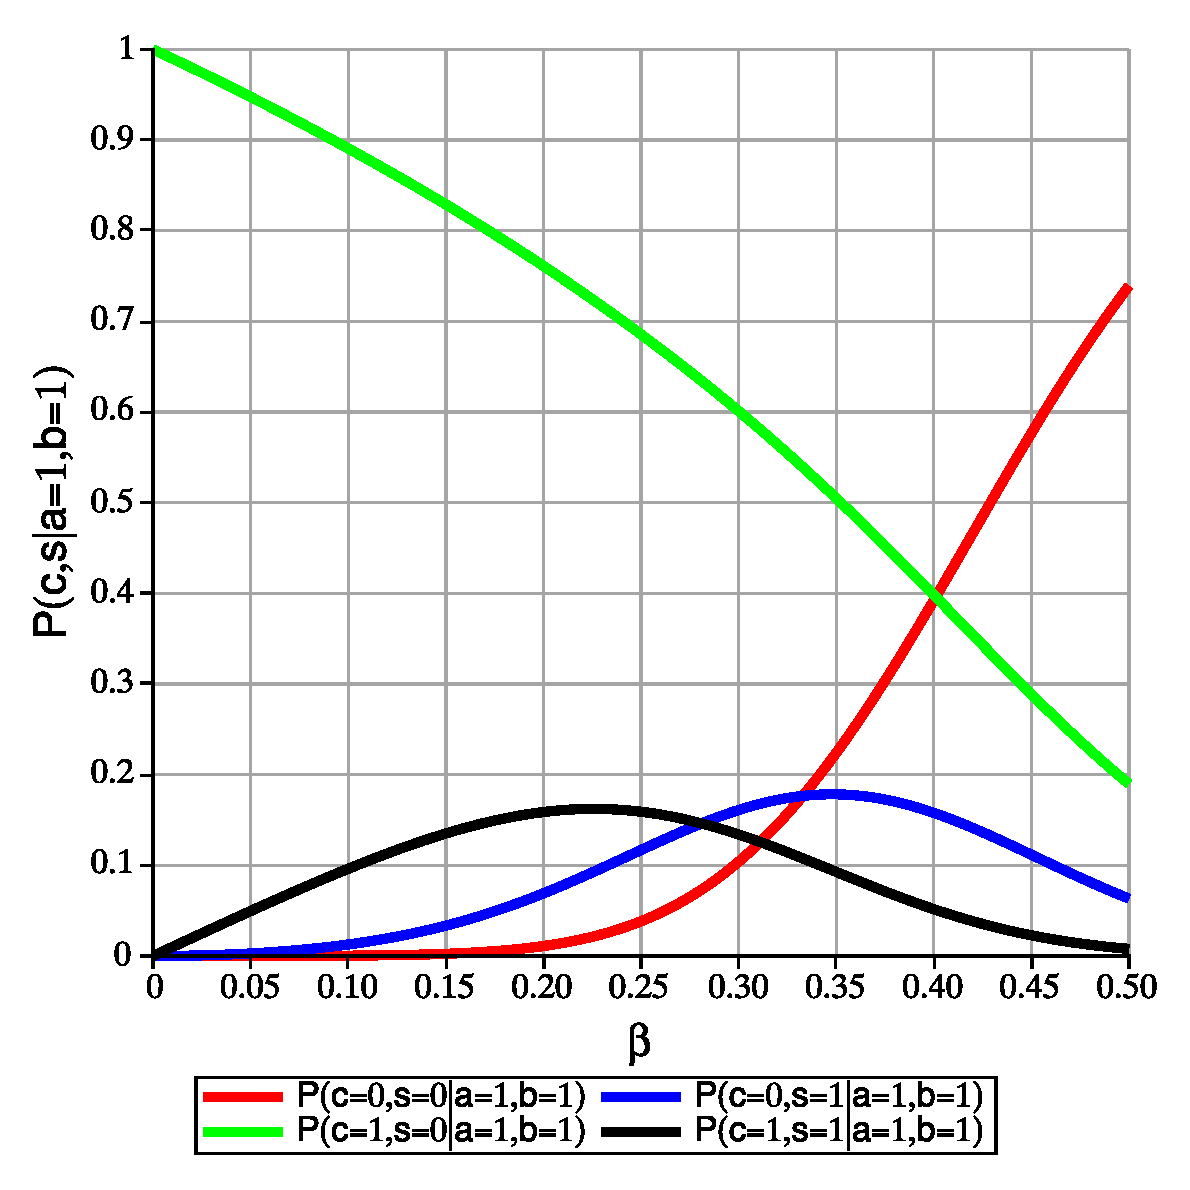
\includegraphics[width=.4\textwidth]{media/noisy_half_adder_16_redundancy_value_dist_11.eps}
        \end{tabular}
    \end{center}
    \caption{Probability distribution for $P(s,c|a,b)$ for the two different cases of $a=1, b=0$ (left)and $a=1, b=1$ (right), respectively. The graphs show the change of the probability distributions as $\beta$ in (\ref{eq:bit_flip_to_0}) varies from $0$ to $\frac{1}{2}$ and $\alpha = 0$; this case is equivalent to assuming there is only leakage of information due to low-voltage. Note the difference to Figure \ref{fig:noise_prob_dist} middle and right. \label{fig:noise_prob_dist_redudancy}}
\end{figure}


\section{Experimental Results}

\section{Conclusion}

\bibliographystyle{unsrtnat}
\bibliography{references} 

\end{document}
